\documentclass[10pt]{article}
\usepackage[letterpaper, margin=1in]{geometry}
\usepackage[pdftex]{graphicx}
\usepackage[utf8]{inputenc}
\usepackage{tikz, wrapfig, amssymb, array, mathtools, circuitikz, physics, parskip, hyperref}
\usepackage{enumerate}
\usepackage{tkz-euclide}
\usepackage{titlesec}
\usepackage{lipsum}
\usepackage[english]{babel}
\usepackage{amsmath, amsthm}
\usepackage{fancyhdr}
\usepackage{xcoffins}
\usepackage{tcolorbox}
\usepackage{../local}


\newcommand{\classcode}{Physics 5C}
\newcommand{\classname}{Introduction to Thermodynamics and Quantum Mechanics}
\renewcommand{\maketitle}{%
\hrule height4pt
\large{Eric Du \hfill \classcode}
\newline
\large{HW 05} \large{\hfill \classname \hfill} \large{\today}
\hrule height4pt \vskip .7em
\normalsize
}
\linespread{1.1}
\begin{document}
    \maketitle

    \section*{Collaborators}

    I worked with \textbf{Andrew Binder} to complete this homework assignment. 

    \section*{Problem 1}

    Show that for $N$ non-interacting spin $\frac{1}{2}$ particles in a magnetic field $B$ the energy $U$ is given by 

    \[ U = -N \mu_B B \tanh\left(\frac{\mu_B B}{k_BT}\right)\]

    the heat capacity is given by 

    \[ \frac{C}{Nk_B} = \left(\frac{\mu_BB}{k_BT}\right)^2 \sech^2\left(\frac{\mu_BB}{k_BT}\right)\]

    and the entropy is given by 

    \[ \frac{S}{Nk_B} = \ln \left[2\cosh \left(\frac{\mu_BB}{k_BT}\right)\right] - \frac{\mu_BB}{k_BT} \tanh \left(\frac{\mu_BB}{k_BT}\right)\]

    \begin{solution} 
        We have from the textbook:

        \begin{align*}
            Z_N &= Z_1^N = 2^{N} \cosh^N( \beta \mu_BB)\\
            \therefore \ln Z_N &= N \ln (2 \cosh (\beta \mu_BB))\\
            &= N \ln 2 + N \ln \cosh(\beta \mu_BB)
        \end{align*}

        Now, let's compute $U = -\frac{\dd \ln Z}{\dd \beta}$: 

        \begin{align*}
            U &= -\frac{\partial \ln Z_N}{\partial \beta}\\
            &= -N \frac{\partial}{\partial \beta} \ln (\cosh(\beta \mu_BB))\\
            &= -N \mu_BB \tanh\left(\frac{\mu_BB}{k_BT}\right) && \text{ computed using WolframAlpha}
        \end{align*}

        Which is exactly the expression that we wanted to derive. Now, since we know that $C = \left(\frac{\partial U}{\partial T}\right)_V$:

        \begin{align*}
            C &= \frac{\partial}{\partial T}\left[- N\mu_B B\tanh\left(\frac{\mu_BB}{k_BT}\right)\right]\\
            &= -N\mu_BB \sech^2\left(\frac{\mu_BB}{k_BT}\right) \cdot \frac{-\mu_BB}{k_BT^2}\\
            &= N \left(\frac{\mu_BB}{T}\right)^2 \cdot \frac{1}{k_B} \sech^2\left(\frac{\mu_BB}{k_BT}\right)\\
            \therefore \frac{C}{Nk_B} &= \left(\frac{\mu_BB}{k_BT}\right)^2 \sech^2\left(\frac{\mu_BB}{k_BT}\right)
        \end{align*}

        Similarly, we know that since $F = -Nk_BT \ln \left( 2\cosh\left(\frac{\mu_BB}{k_BT}\right)\right)$, then:

        \begin{align*}
            S = \frac{U - F}{T} &= \frac{1}{T} \left[ -N\mu_BB \tanh\left(\frac{\mu_BB}{k_BT}\right) + Nk_BT \ln \left[2\cosh\left(\frac{\mu_BB}{k_BT}\right) \right]\right]\\
            &= \frac{Nk_BT}{T} \left[-\frac{\mu_BB}{k_BT}\tanh\left(\frac{\mu_BB}{k_Bt}\right) + \ln \left[2\cosh\left(\frac{\mu_BB}{k_BT}\right)\right]\right]\\
            \therefore \frac{S}{Nk_B} &= \ln \left[2\cosh \left(\frac{\mu_BB}{k_BT}\right)\right] - \frac{\mu_BB}{k_BT} \tanh \left(\frac{\mu_BB}{k_BT}\right)
        \end{align*}

        And so we're done. $\blacksquare$
    \end{solution}

    \pagebreak

    \section*{Problem 2}

    A certain magnetic system contains $n$ independent molecules for unit volume, each of which has four energy levels given by $0$, $\Delta - g\mu_B B$, $\Delta$, $\Delta + g\mu_BB$ ($g$ is a constant). Write down the partition function, compute teh Helmholtz function and hence compute the magnetization $M$. Hence show that the magnetic susceptibility $\chi$ is given by 
    
    \[ \chi = \lim_{B \to 0} \frac{\mu_0M}{B} = \frac{2 n \mu_0 g^2 \mu_B^2}{k_BT (3 + e^{\Delta/k_BT})}\]

    \begin{solution}
        The partition function is defined as $Z = \sum e^{-\beta E_i}$, so if we substitute in the energies we get:

        \[Z = 1 + e^{-\beta\Delta + \beta g\mu_BB} + e^{-\beta \Delta} + e^{-\beta \Delta - \beta g\mu_BB}\]

        So therefore, since $F = -nk_BT \ln Z$, then 

        \[ F = -nk_BT \ln (1 + e^{-\beta\Delta + \beta g\mu_BB} + e^{-\beta \Delta} + e^{-\beta \Delta - \beta g\mu_BB})\]

        From here, it's useful to rewrite the partition function as: 

        \[ Z = 1 + e^{\beta \Delta} \left(1 + 2 \cosh \left(\frac{g\mu_BB}{k_BT}\right)\right)\]

        Now, the magnetization $M$ is defined as $M = -\left(\frac{\partial F}{\partial B}\right)_T$, so if we take the derivative of $F$: 


        \begin{align*}
            M &= nk_BT \frac{\partial}{\partial B} \left(\ln \left[ 1 + e^{-\beta \Delta}\left( 1 + 2\cosh\left(\frac{g \mu_BB}{k_BT}\right)\right)\right]\right)\\
            &= nk_BT\frac{\frac{1}{k_BT} 2g\mu_B  \sinh\left(\frac{g\mu_BB}{k_BT}\right)}{2 \cosh \left(\frac{g\mu_BB}{k_BT}\right) + 1 + e^{\beta \Delta}}
        \end{align*}

        The derivative was computed by hand then checked using WolframAlpha. Since we're on the order of molecules, it's appropriate to assume that $\sinh x \approx x$ and $\cosh x \approx 1$:

        \begin{align*}
            M &= \frac{2n g^2 \mu_B \left(\frac{g\mu_BB}{k_BT}\right)}{ 3 + e^{\beta \Delta}}\\
            &= \frac{2ng^2\mu_B^2 B}{k_BT(3 + e^{\beta \Delta})}
        \end{align*}

        Now we can compute the limit:

        \begin{align*}
            \chi &= \lim_{B \to 0} \frac{\mu_0 M}{B} = \lim_{B \to 0}\frac{\mu_0}{B} \frac{2ng^2\mu_B^2 B}{k_BT(3 + e^{\beta \Delta})}\\
            &= \frac{2 n \mu_0 g^2 \mu_B^2}{k_BT (3 + e^{\Delta/k_BT})}
        \end{align*}

        And so we're done. $\blacksquare$


        % Before we take the limit, it's useful to write rewrite the partition function into:

        % \[ Z = 1 + e^{\beta \Delta} \left(1 + 2 \cosh \left(\frac{g\mu_BB}{k_BT}\right)\right)\]

        % So now taking the limit: 

        % \begin{align*}
        %     \chi &= \lim_{B \to 0} \frac{\mu_0 M}{B}\\
        %     &= \lim_{B \to 0} \frac{nk_BT} \beta g \mu_B
        % \end{align*}
    \end{solution}

    \pagebreak
    \section*{Problem 3}

    The energy $E$ of a system of three independent harmonic oscillators is given by 

    \[ E = \left(n_x + \frac{1}{2}\right) \hbar \omega + \left(n_y + \frac{1}{2}\right) \hbar \omega + \left(n_z + \frac{1}{2}\right) \hbar \omega\] 

    Show that the partition function $Z$ is given by 

    \[ Z = Z_{SHO}^3\]
    
    where $Z_{SHO}$ is the partition function of a simple harmonic oscillator given in eqn. 20.3. Hence show that the Helmholtz function is given by:

    \[ F = \frac{3}{2} \hbar \omega + 3k_BT\ln (1 - e^{-\beta \hbar \omega})\] 

    and that the heat capacity tends to $3k_B$ at high temperature.


    \begin{solution}
        Call $E = E_x + E_y + E_z$ for the $n_x$, $n_y$ and $n_z$ components. Now we write out the partition function: 

        \begin{align*}
            Z &= \sum e^{-\beta(E_x + E_y + E_z)}\\
            &= \sum e^{-\beta E_x} e^{-\beta E_y} e^{-\beta E_z}
        \end{align*}

        Now notice that since $x, y, z$ are orthogonal, we can actually combine them under a common $n$. Therefore:

        \[ Z = \sum e^{-3\beta E_x} = Z_{SHO}^3\]

        Now to show the Helmholtz function, we use the fact that $F = -k_BT \ln Z$:

        \begin{align*}
            F &= -k_BT \ln Z_{SHO}^3\\
            &= -3k_BT \ln Z_{SHO}\\
            &= 3\left(\frac{\hbar \omega}{2} + k_BT \ln (1- e^{-\beta \hbar \omega})\right)\\
            &= \frac{3}{2} \hbar \omega + 3k_BT\ln (1 - e^{-\beta \hbar \omega})
        \end{align*}

        Note that $\ln Z_{SHO} = \left(\frac{\hbar \omega}{2} + k_BT \ln (1- e^{-\beta \hbar \omega})\right)$ is given in the textbook, which is what I used to simplify this expression. Now to compute the heat capacity, we first have 

        \[ U = \frac{3\hbar \omega}{2} + \frac{3\hbar \omega}{e^{\beta \hbar \omega} - 1}\]

        So therefore, we take the derivative with respect to $T$: 

        \begin{align*}
            \frac{\partial U}{\partial T} &= 3\hbar \omega \frac{\frac{\hbar \omega}{k_BT} e^{\hbar \omega/k_BT}}{T^2\left(e^{\hbar \omega/k_BT} -1\right)^2}\\
            &= 3k_B(\beta \hbar \omega)^2\frac{e^{\beta \hbar \omega}}{\left(e^{\beta \hbar \omega} - 1\right)^2}
        \end{align*}


        And we know that at high temperatures, $e^{\beta \hbar \omega} - 1 \approx \beta \hbar \omega$ (by a Taylor expansion). therefore, 

        \begin{align*}
            \frac{\partial U}{\partial T} &= 3k_B(\beta \hbar \omega)^2 \frac{e^{\beta \hbar \omega}}{(\beta \hbar \omega)^2}\\
            &= 3k_B
        \end{align*}

        As desired. $\blacksquare$
    \end{solution}

    \pagebreak
    \section*{Problem 4}

    The internal levels of an isolated hydrogen atom are given by $E = -R/n^2$ where $R = 13.6$eV. the degeneracy of each level is given by $2n^2$. 

    \begin{enumerate}[(a)]
    \item Sketch the energy levels
    
    \begin{solution}
        A sketch is shown below: 

        \[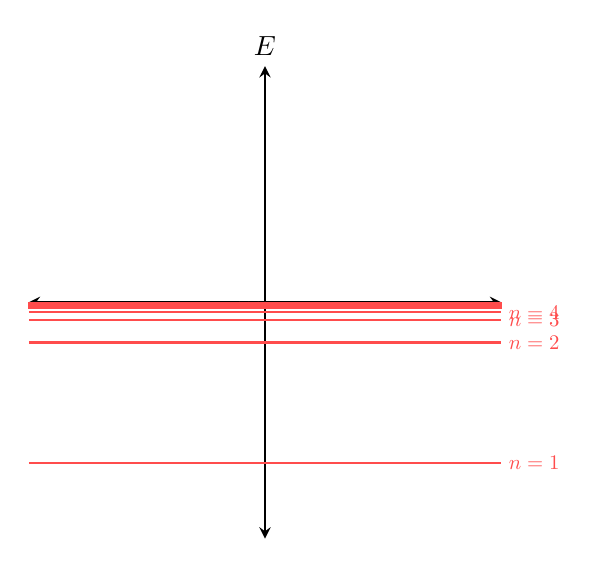
\begin{tikzpicture}[scale=0.15]
            \draw[thick, stealth-stealth] (-20,0) -- (20,0);
            \draw[thick, stealth-stealth] (0,-20) -- (0,20) node[anchor=south] {$E$};
            \draw[thick, red!70] (-20,-13.6) -- (20,-13.6) node[scale=0.75, anchor=west] {$n = 1$};
            \draw[thick, red!70] (-20,-3.4) -- (20,-3.4) node[scale=0.75, anchor=west] {$n = 2$};
            \draw[thick, red!70] (-20,-1.5111) -- (20,-1.5111) node[scale=0.75, anchor=west] {$n = 3$};
            \draw[thick, red!70] (-20, -0.85) -- (20,-0.85) node[scale=0.75, anchor=west] {$n = 4$};
            \filldraw[red!70] (-20,-0.544) -- (20,-0.544) -- (20,-0.001) -- (-20,-0.001) -- cycle node[scale=0.75, anchor=west] {$\dots$};
        \end{tikzpicture}\] 


        As we can see, the energy levels approach $E = 0$, which makes sense since as $n \to \infty$, $E \propto 1/n^2$ so $E \to 0$. Thanks to \textbf{Andrew Binder} for the Ti\textit kZ diagram.
    \end{solution}
    \item Show that 
    
    \[ Z = \sum_{n = 0}^\infty 2n^2 \exp{\frac{R}{n^2k_BT}}\]

    \begin{solution}
        Summing over the energy levels, we get 

        \[ Z = \sum_n e^{-\beta E_n} = \sum_1^\infty 2n^2 e^{\beta R/n^2} = \sum_1^\infty 2n^2e^{\frac{R}{n^2k_BT}} = \sum_{n = 0}^\infty 2n^2 \exp{\frac{R}{n^2k_BT}}\]

        And so we're done. $\blacksquare$
    \end{solution}
    \end{enumerate}
\end{document}